%% Equipe:
%% Leonardo Winter Pereira
%% Geanine Inglat
%% André Eleutério

%% Tema:
%% The Propeller Clock

\documentclass[openright]{normas-utf-tex} %openright = O capítulo começa sempre em páginas ímpares
%\documentclass[oneside]{normas-utf-tex} %oneside = Para dissertações com número de páginas menor que 100 (apenas frente da folha)

\usepackage[alf,abnt-emphasize=bf,bibjustif,recuo=0cm, abnt-etal-cite=2, abnt-etal-list=99]{abntcite} %configuração correta das referências bibliográficas.
\usepackage[brazil, portuges]{babel} % pacote português brasileiro
\usepackage[utf8]{inputenc} % pacote para acentuação direta
\usepackage{amsmath,amsfonts,amssymb} % pacote matemático
\usepackage{graphicx} % pacote gráfico
\usepackage{times} % fonte times
\usepackage{url} % fonte times
\usepackage{listings} % pacote para códigos


%\geometry{left=3.0cm,right=1.5cm,top=4cm,bottom=1cm}       Usado para realizar pequenos ajustes das margens.

% ---------- Preâmbulo ----------
\instituicao{Universidade Tecnológica Federal do Paraná} % nome da instituição
\programa{Curso em Engenharia de Computação} % nome do programa

\documento{Monografia} % [Dissertação] ou [Tese]
\nivel{Graduando} % [Mestrado] ou [Doutorado]
\titulacao{Oficinas de Integração II} % [Mestre] ou [Doutor]

\titulo{\MakeUppercase{Relógio com Varredura Mecânica}} % Título do trabalho em português
\title{\MakeUppercase{The Propeller Clock}} % Título do trabalho em inglês

\autor{Leonardo Winter Pereira, Geanine Inglat, André Eleutério} % Autor do trabalho
\cita{PEREIRA, Leonardo; INGLAT, Geanine; ELEUTÉRIO, André} % sobrenome (maiúsculas), Nome do autor do trabalho

\palavraschave{Relógio com Varredura Mecânica, Arduino, LED} % Palavras-chave do trabalho
\keywords{Propeller Clock, Arduino, LED} % Palavras-chave do trabalho em inglês

\comentario{\UTFPRdocumentodata\ apresentada ao \UTFPRprogramadata\ da \ABNTinstituicaodata\ como requisito parcial para aprovação na disciplina de "\UTFPRtitulacaodata\ ".}

\orientador{César Manuel Vargas Benitez} % nome do orientador do trabalho
\local{Curitiba} % cidade
\data{\the\year} % ano automático

%---------- Inicio do Documento ----------
\begin{document}

\capa % Geração automática da capa
\folhaderosto % Geração automática da folha de rosto

%resumo
%\begin{resumo}

%\end{resumo}

%abstract
%\begin{abstract}

%Abstract text (maximum of 500 words).

%\end{abstract}

% listas (opcionais, mas recomenda-se a partir de 5 elementos)
\listadefiguras % Geração automática da lista de figuras
\listadetabelas % Geração automática da lista de tabelas
\listadesiglas % Geração automática da lista de siglas
\listadesimbolos % Geração automática da lista de símbolos

% sumário
\sumario % Geração automática do sumário

%---------- Início do Texto ----------
%---------- Primeiro Capitulo ----------
\chapter{Introdução}
\label{chap:intro}

O propeller clock depende de um fenômeno chamado \sigla{POV}{Persistência da visão} (Persistence of vision, em inglês). Persistência da visão consiste no fenômeno observado quando um objeto visto pelo olho humano persiste na retina por uma fração de segundo após a sua percepção. Assim, imagens projetadas com uma frequência superior a 16Hz associam-se na retina sem interrupção~\cite{Wikipedia2013}~\cite{Anderson1993}.

Segundo essa teoria, ao captar uma imagem, o olho humano levaria uma fração de tempo para "apagá-la". Assim, quando os quadros de um filme de cinema são projetados na tela, o olho mistura o quadro anterior com o seguinte, provocando a ilusão de movimento: um objeto colocado à esquerda num quadro, aparecendo à direita no quadro seguinte, cria a ilusão de que o objeto se desloca da esquerda para a direita.

Posteriormente foi comprovado que este fenômeno é mais complexo, e melhor explicado quando divido entre Movimento \simbolo{$\phi$}{Phi} e Movimento \simbolo{$\beta$}{Beta}, pelo psicólogo checo Max Wertheimer. Porém esta análise fisiológica da visão foge do escopo desse trabalho~\cite{Kaufman1974}.

A persistência da visão pode ser observada no cotidiano ao se ligar um ventilador. Assim que o ventilador acelera, não é possível ver as hélices individualmente, somente um círculo.

Isso se aplica ao nosso trabalho pois ao rotacionar rapidamente uma hélice com diversos \sigla{LED}{Diodo emissor de luz}s, e ao coordenar o acendimento dos mesmos, é possível produzir imagens claramente visíveis ao olho humano.

\section{Componentes} %GEANINE
%Lista dos componentes utilizados e custo aproximado de cada um
A tabela 1 mostra uma relação dos materiais necessários para a confecção do display de varredura mecânica.

\begin{table}[!h]
	\centering
	\label{tab:lista-materiais-propeller}
	\begin{tabular}{ccc}
		\hline
		Produto & Quantidade & Valor (Individual) \\
		\hline
		Arduino Nano & 1 & R\$44,00 \\
		Latch 74LS373 & 1 & R\$1,85 \\
	    Regulador de tensão 5V - 7805 & 1 & R\$1,00 \\
		Capacitor 47\simbolo{$\mu$}{micro}F & 1 & R\$0,75 \\
        Cristal 40MHz & 1 & R\$0,70 \\
        Matriz de Resistores 330{$\Omega$} & 2 & R\$0,08 \\
        LED RGB & 16 & R\$1,10 \\
        Barra de Pinos 28 pinos & 1 & R\$0,60 \\
        Barra de Pinos 20 pinos & 2 & R\$0,60 \\
        Diodo emissor IR & 1 & R\$0,80 \\
        Fototransistor & 1 & R\$0,80 \\
        Barra de pinos 30 pinos & 1 & R\$0,60 \\
        Matriz de Contatos de Cobre & 1 & R\$8,90 \\
        Cooler 3800 RPM & 1 & R\$9,10 \\
        Slot Bateria 9V & 1 & R\$---- \\
        Total & - & R\$88.06 \\
		\hline
	\end{tabular}
    \caption[Orçamento para o Display de Varredura Mecânica]{Orçamento para o Display de Varredura Mecânica}
\end{table}


Além do desenvolvimento do display de varredura mecânica, foi necessário desenvolver um Tacômetro digital para Arduino, para ser possível testar a frequência do Cooler utilizado no projeto. Entretanto, este dispositivo será apenas utilizado como ferramenta de desenvolvimento, não fazendo parte da versão final do mesmo.

A lista de materiais para este projeto está listada na tabela 2:

\begin{table}[!h]
	\centering
	\label{tab:lista-materiais-tacometro}
	\begin{tabular}{ccc}
		\hline
		Produto & Quantidade & Valor (Individual) \\
		\hline
		Arduino Nano & 1 & R\$44,00 \\
	    Trimpot 5k\simbolo{$\Omega$}{Omega} & 1 & R\$0,58 \\
        Barra de pinos 30 pinos & 1 & R\$0,60 \\
        Transistor NPN 2n2222 & 2 & R\$0,25 \\
        LED IR & 1 & R\$0,80 \\
        Fototransistor & 1 & R\$0,80 \\
        Resistor 10{$\Omega$} & 1 & R\$0,08 \\
        Resistor 100k{$\Omega$} & 1 & R\$0,08 \\
        Resistor 15k{$\Omega$} & 1 & R\$0,08 \\
        Protoboard & 1 & R\$86,90 \\
        Total & - & R\$134,42 \\
		\hline
	\end{tabular}
    \caption[Lista de materiais utilizados no Tacômetro Digital]{Lista de materiais utilizados no Tacômetro Digital}
\end{table}

%b) "Quais partes constituem o dispositivo e como interagem entre si?" (utilizar um diagrama de blocos como auxiliar na descrição)
Uma breve descrição dos principais componentes que constituem o projeto será realizada neste momento:

\begin{itemize}
\item Arduino Nano: Será utilizado para realizar todo o processamento de informações necessário no projeto, como por exemplo, o cálculo do número de rotações da hélice, o controle dos LEDs, entre outros.
\item Latch 74LS373: Circuito integrado responsável por controlar o acendimento dos LEDs. Este componente é necessário devido ao baixo número de portas de saída por parte do Arduino.
\item Regulador de tensão 5V – 7805: O regulador de tensão é necessário para poder limitar a tensão nos LEDs, pois a diferença de potencial necessária nestes componentes é menor do que é necessário no cooler.
\item Capacitor 47 {$\mu$}F: Utilizado como filtro no regulador de tensão.
\item Cristal 40MHz: Utilizado para contar o tempo corretamente no relógio.
\item Matriz de Resistores 330{$\Omega$}: Utilizada para regular a corrente que vai para os LEDs
\item LED RGB: Utilizados para criar o efeito de ilusão de óptica ao acenderem nos momentos certos.
\item Socket 28 pinos: Utilizados para poder fixar o Arduino na matriz de contato.
\item Diodo emissor IR e Fototransistor: Utilizados para realizar a contagem de rotações por minuto do cooler.
\item Cooler 3800 RPM: Melhor escolha para o motor pois já possui um circuito pronto de potência e velocidade. Deve ser de no mínimo 3600 rpm para criar um bom efeito visual.
\end{itemize}

\section{Conteúdos Envolvidos} %LEONARDO

Para o desenvolvimento deste projeto, diversos são os conhecimentos necessários envolvendo diferentes áreas, desde eletrônica e programação até a física envolvida por trás de alguns aspectos da visão.

Na área de eletrônica, é necessário compreender os seguintes aspectos:
\begin{itemize}
\item Sensores IR: Existem sensores de infravermelho ativos e passivos. Um sensor de infravermelho ativo é composto por um emissor de luz infravermelha e um receptor, que reage a essa luz. Por sua vez, um sensor de infravermelho passivo não emite luz infravermelha, mas apenas capta esse tipo de luz no ambiente~\cite{RoboLivre2014}.

    Neste projeto, usaremos sensores de infravermelho para medir as rotações do relógio.
\item Construção da \sigla{PCI}{Placa de Circuito Impresso}: Será necessária a contrução de uma placa de circuito impresso para o projeto. Nela estarão contidos, entre outros componentes, os LEDs, posicionados da maneira correta para a visualização otimizada da saída do projeto. É necessária a compreensão de todos os passos para a criação da matriz.
\end{itemize}

Na área de programação, é fundamental compreender como programar o Arduino, pois é ele quem controla o acendimento dos LED's~\cite{Arduino2014}~\cite{ArduinoRef2014}.

Na área de mecânica é imprescindível o cálculo exato das rotações do motor. Erros, mesmo que pequenos, nesta etapa são suficientes para que a imagem final seja diferente do esperado.

Entretanto, a principal preocupação será com conceitos de POV e cadência, uma vez que abrangem a parte principal do projeto: o objetivo de causar uma ilusão aos olhos do espectador para criar uma imagem~\cite{Anderson1993}.

	O projeto também envolve conhecimento na área de eletrônica e programação, é preciso desenvolver hardware e software que apliquem corretamente os conceitos teóricos estudados. O primeiro projeto similar desenvolvido foi feito em 1995 por Bob Blick e será utilizado como referência para o desenvolvimento deste trabalho~\cite{Blick2002}.

\section{Metodologia de Execução} %TODOS JUNTOS

%a) Quais são as tarefas *específicas'* necessárias para a execução do projeto? Descrever brevemente o que envolve cada tarefa.
%b) Quais as relações de dependência entre as tarefas?
%c) Quanto tempo está previsto para cada tarefa (estimativa)?
%Sugestão: utilizar um diagrama Gantt

Será necessário construir peças, realizar testes e desenvolver o software do projeto. Construiremos um tacômetro, um motor para rotacionar a placa e uma matriz de contatos.
A construção do motor depende da construção do tacômetro, enquanto o desenvolvimento do software depende de toda a parte de hardware estar pronta pois testes são fundamentais durante o processo de desenvolvimento.

A duração de cada tarefa varia, com algumas durando apenas um dia e outras mais de uma semana. A tarefa que mais levará tempo é a redação da monografia, pois será feita com o decorrer do projeto.

O diagrama de blocos, utilizado para demonstrar de forma simples a relação entre cada componente do projeto, está mostrado na Figura 1.

\begin{figure}[!h]
	\centering
	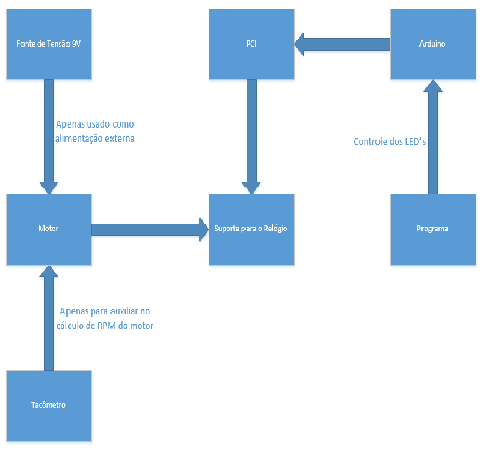
\includegraphics{./Diagrama_Blocos.png}
	\caption[Diagrama de Blocos do projeto]{Diagrama de Blocos do projeto}
	\label{fig:Diagrama_Blocos}
\end{figure}

\begin{itemize}
\item Construção do tacômetro:
Serão usados um LED infravermelho e um receptor infravermelho, além do cooler onde serão posicionados. Com esse sistema é possível contar quantas vezes o sinal é cortado pelas hélices do cooler, e assim podemos calcular o número de rotações por minuto do sistema. Os cálculos serão efetuados com um arduino.
\item Construção da matriz de contatos:
São duas etapas, o design e a construção. No design será desenhado como a placa será impressa e onde irão os componentes. Na construção, produziremos a placa com peróxido e depois soldaremos os componentes nela.
\item Construção do motor:
Para construir o motor, as hélices do motor serão removidas e o motor será fixado em uma base com uma fonte de alimentação.
\item Integração das peças de hardware:
Para poder prosseguir com o projeto e finalizar o hardware, a matriz de contatos, o motor e o Arduino serão integrados.
\item Desenvolvimento do software:
Será desenvolvido um algoritmo que coordene o acender e apagar dos LEDs para que, ao girarem, formarão uma imagem. O arduino será programado. Para programar, usaremos uma interface no computador que nos permite programar em C e passar esse código para o arduino através da uma porta USB.
\end{itemize}

O diagrama de Gantt do projeto, com as principais tarefas especificadas, está mostrado na figura 2.

\begin{figure}[!h]
	\centering
	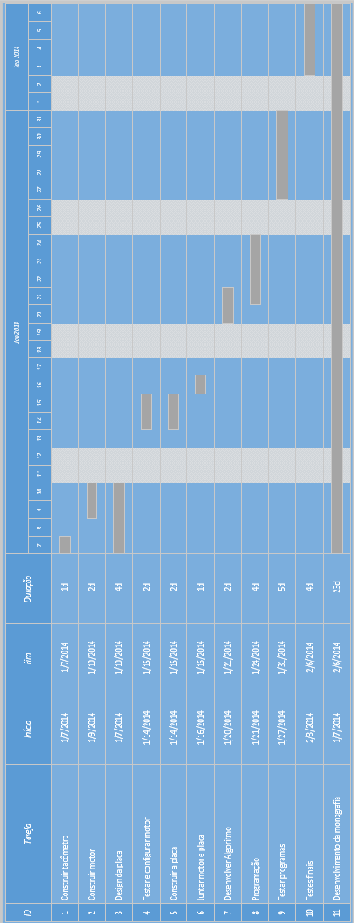
\includegraphics{./Diagrama_Gantt.png}
	\caption[Diagrama de Gantt do projeto]{Diagrama de Gantt do projeto}
	\label{fig:Diagrama_Gantt}
\end{figure}

\section{Banca Examinadora}
\begin{itemize}
\item Aluno convidado:
Iuri Barcat
\item Professor Orientador:
César Benitez (DAELN)
\item Professora convidada:
Leyza Dorini (DAINF)
\item Professor da disciplina:
Hugo Vieira Neto
\end{itemize} 
%---------- Segundo Capitulo ----------
\chapter{Metodologia}
\label{chap:desen}

Nesta seção será apresentado o desenvolvimento de todo o projeto, na ordem que o mesmo foi criado. Desta forma fica mais fácil para o leitor entender o desenvolvimento do projeto, além de poder ser utilizado como base para projetos futuros mais facilmente.

\section{Construção do Tacômetro Digital}
Um tacômetro não é nada mais que um frequencímetro modificado. Enquanto este mede a frequência de uma onda, aquele é capaz de medir a frequência de um objeto (desde que este objeto realize rotações).

A forma mais fácil de se construir tal ferramenta é utilizando dois LED's infravermelhos, um receptor e outro emissor. Inicialmente, a conexão entre os dois está alta (ativa), e quando esta conexão se torna baixa (inativa) significa que algo cortou o sinal entre os dois LED's. Desta forma, podemos desenvolver um algoritmo para contar quantas vezes este sinal é cortado em um minuto, podendo determinar a frequência do motor utilizado no projeto.

O diagrama esquemático deste projeto é simples, e será apresentado na figura 3.

\begin{figure}[!h]
	\centering
	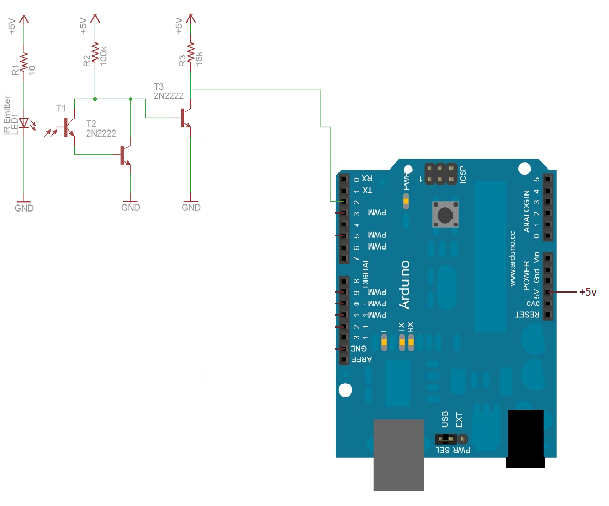
\includegraphics{./tachometer_schematic.png}
	\caption[Diagrama Esquemático do Tacômetro Digital]{Diagrama Esquemático do Tacômetro Digital}
	\label{fig:tachometer_diagram}
\end{figure}

Um cuidado especial que teve que ser tomado é a posição dos LED's. É importante que estes estejam a uma certa distância um do outro, mas não muito afastados, e também perfeitamente alinhados, para que o sinal recebido pelo LED receptor seja alto o suficiente para manter todo o sistema em alto, enquanto o motor não cortá-lo. Uma distância razoável é mostrada na figura 4.

\begin{figure}[!h]
	\centering
	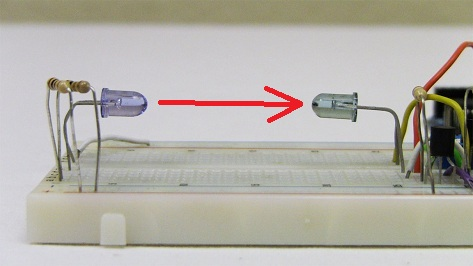
\includegraphics{./break__beam_small.jpg}
	\caption[Distância razoável para os LED's]{Distância razoável para os LED's}
	\label{fig:break__beam_small}
\end{figure}

Com o hardware feito, foi necessário desenvolver um algoritmo para a contagem da frequência. Vale lembrar que o próprio Arduino possui diversas bibliotecas e funções que facilitaram o desenvolvimento do nosso algoritmo. A função attachInterrupt(), por exemplo, é chamada no momento que uma interrupção no sistema existe~\cite{Arduino_attachInterrupt()}.

\begin{lstlisting}
volatile float time = 0;
volatile float time_last = 0;
volatile int rpm_array[5] = {0,0,0,0,0};

void setup()
{
  //Pino Digital 2 foi definido como interruptor
 attachInterrupt(0, fan_interrupt, FALLING);

  // Mensagem no prompt de comando do Arduino
  Serial.print("Current RPM:");
}

//Funcao Loop que calcula a RPM do motor e atualiza
//este valor na saida Serial
void loop()
{
    int rpm = 0;

    while(1)
    {
        //Define a velocidade de atualizacao da contagem
        delay(400);

        Serial.print("                ");

        //Atualiza a contagem do RPM
        Serial.print(rpm);

        //Atualiza o RPM
        if(time > 0)
        {
            //Para obtermos um valor mais proximo do real, utili-
            //zaremos uma media entre 5 medicoes consecutivas
            rpm_array[0] = rpm_array[1];
            rpm_array[1] = rpm_array[2];
            rpm_array[2] = rpm_array[3];
            rpm_array[3] = rpm_array[4];

            //4 e o numero de helices do motor
            rpm_array[4] = 60*(1000000/(time*4));

            rpm = (rpm_array[0] + rpm_array[1] + rpm_array[2]
            + rpm_array[3] + rpm_array[4]) / 5;
        }
    }
}

//Ponto que o sinal entre os dois LED's e cortado pelo motor
void fan_interrupt()
{
   time = (micros() - time_last);
   time_last = micros();
}
\end{lstlisting}

Com isto, foi possível determinar a velocidade do motor de 2400 rpm ou uma frequência de 40 Hz.

\section{Construção do Motor}
Um ponto chave no desenvolvimento do projeto foi encontrar uma solução para girar a PCI com uma velocidade suficiente para gerar o efeito de persistência da visão com uma resolução que fosse agradável aos olhos.
Para tal, escolhemos utilizar coolers de gabinete de computador. Em um primeiro momento testamos um cooler pequeno, com alimentação de 12 V. Ele girava a placa (uma protoboard, em uma fase bem primitiva dos testes) com uma velocidade muito abaixo do esperado. Além disse foi necessário quebrar a parte plástica que cobria o cooler para podermos conectar a placa à peça central giratória.
Como a velocidade deste cooler não foi suficiente, pesquisamos e compramos um cooler com alimentação de 127~230V, da marca Ultrar. Este cooler é mostrado na figura 5.

\begin{figure}[!h]
	\centering
	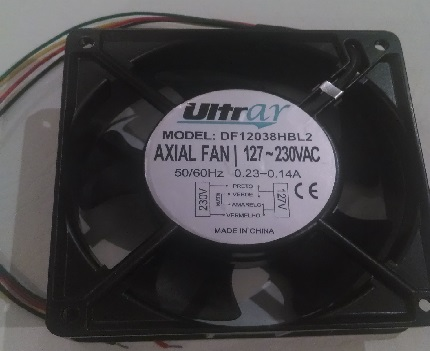
\includegraphics{./cooler1.jpg}
	\caption[Cooler utilizado no projeto final]{Cooler utilizado no projeto final}
	\label{fig:cooler_Ultrar}
\end{figure}


Utilizamos 127V, e a velocidade de rotação atingiu o nível que tínhamos em mente. Porém, com este cooler mais potente, o problema de conectar a placa na parte giratória era mais difícil de ser resolvido pois, ao contrário do cooler de 12V que era revestido por plástico, esse cooler é revestido por uma placa de metal maciço. Como esse cooler gira tão rápido que chega a ser perigoso para quem o está manejando, decidimos manter essa peça de metal e criar uma solução para conseguir manter a protoboard fixa à peça giratória. Era necessário elevar a placa aproximadamente 15 mm da peça giratória. Isso se dá ao fato de que a proteção é um pouco mais alta que a peça giratória, e isso causaria atrito entre a placa e a proteção. Esta proteção é mostrada na figura 6.

\begin{figure}[!h]
	\centering
	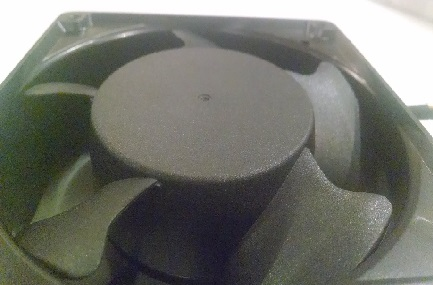
\includegraphics{./cooler2.jpg}
	\caption[Proteção do cooler]{Proteção do cooler}
	\label{fig:cooler_protecao}
\end{figure}

Em um primeiro momento, foi decidido soldar a bateria que alimenta o Arduino na própria placa de LEDs e depois criar um contrapeso para que não ficasse instável. Como a bateria cabe dentro da parte redonda do cooler, ao colocá-la ali conseguimos resolver dois problemas: o do contrapeso da placa e o da elevação em relação à proteção. Portanto a bateria foi fixada em cima da parte central do cooler e a placa em cima da bateria.

\section{Construção da PCI}
A  parte eletrônica do projeto envolvia criar uma placa onde todos os 17 LEDs estivessem conectados ao Arduino e funcionando.

Primeiramente, é importante mostrar o esquemático, utilizado como base para o desenvolvimento da placa. Este esquemático é apresentado na figura 7.

\begin{figure}[!h]
	\centering
	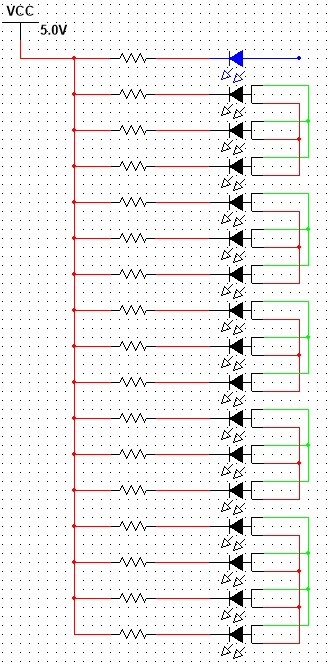
\includegraphics{./esquematico.jpg}
	\caption[Esquemático base para a solda]{Esquemático base para a solda}
	\label{fig:esquematico}
\end{figure}

Em um primeiro momento utilizamos uma protoboard para montar protótipos, porém rapidamente vimos como esta era uma solução inadequada devido ao peso e espessura de tal componente. Então utilizamos uma matriz de contatos para posicionar os LEDs, resistores e Arduino. Isso nos dava maior flexibilidade com o posicionamento das peças além de ser muito leve e ter espessura desprezível.

Como mencionado anteriormente, a bateria foi posicionada diretamente no cooler, portanto não houve necessidade de nos preocuparmos com contrapeso. Já os LEDs foram posicionados alinhados, com resistores à esquerda e o Arduino abaixo, como apresentado na figura 8.

\begin{figure}[!h]
	\centering
	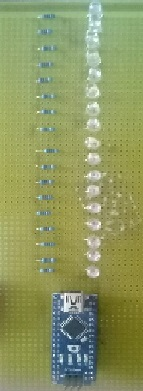
\includegraphics{./placa_cima.jpg}
	\caption[Estado final da Matriz de Contatos]{Estado final da Matriz de Contatos}
	\label{fig:placa_cima}
\end{figure}

A solda final da matriz de contatos ficou como mostrada na figura 9.

\begin{figure}[!h]
	\centering
	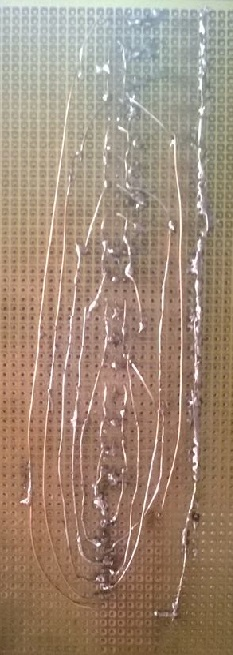
\includegraphics{./placa_baixo.jpg}
	\caption[Solda da Matriz de Contatos]{Solda da Matriz de Contatos}
	\label{fig:placa_cima}
\end{figure}

Após a finalização da solda, foi verificado que, se a a matriz de contatos fosse realmente utilizada, correríamos o risco de algum ponto de solda se soltar, ou até mesmo ocorrer um curto-circuito no sistema. Desta forma, decidimos descartar a matriz de contatos e desenvolver uma PCI. Os resultados finais serão vistos nas figuras 10 e 11.

\begin{figure}[!h]
	\centering
	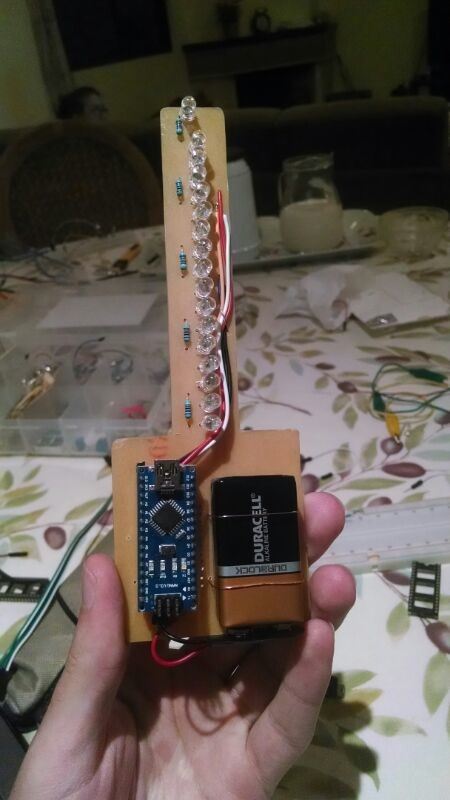
\includegraphics{./PCI_cima.jpg}
	\caption[PCI vista de cima]{PCI vista de cima}
	\label{fig:pci_cima}
\end{figure}

\begin{figure}[!h]
	\centering
	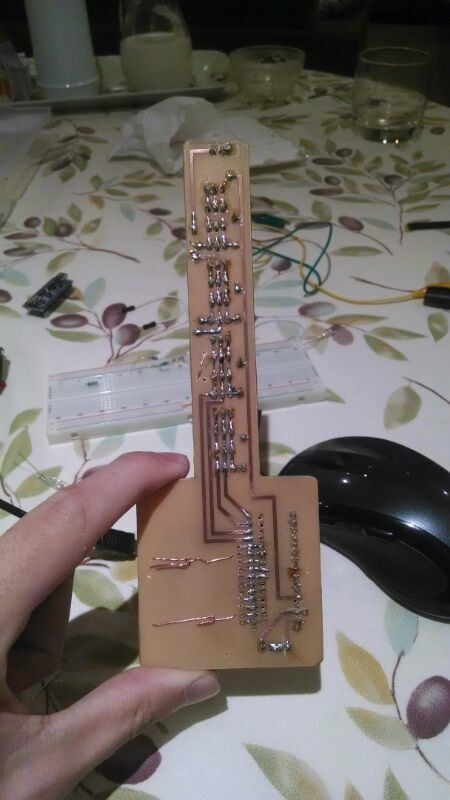
\includegraphics{./PCI_baixo.jpg}
	\caption[PCI vista de baixo]{PCI vista de baixo}
	\label{fig:pci_baixo}
\end{figure}

Vale ressaltar que, com o desenvolvimento da PCI, a bateria também mudou de lugar, para facilitar o carregamento ou até mesmo uma troca desta, caso haja necessidade.

Com a PCI criada, pudemos começar a nos preocupar com o controle dos LED's por parte do Arduino, tendo em vista o baixo número de portas deste e o alto número de LED's do relógio.
Como a velocidade de rotação varia com a distância relativa ao ponto que gira, era necessário controlar os LEDs separadamente. Se todos piscassem ao mesmo tempo haveria uma diferença perceptível e os ponteiros do relógio ficariam destorcidos. Para resolver esse problema dividimos os LEDs em 6 grupos.
O primeiro LED era controlado individualmente e ligado apenas à uma porta do Arduino. Este LED é o que gera os pontos fixos que marcam os minutos do relógio.
Os outros 16 LEDs foram divididos em 4 grupos de 3 e um de 4 LEDs cada.

Essa proporção foi escolhida pois era necessário reservar duas porta do Arduino para cada grupo, e esta limitação foi o que nos levou a dividí-los desta maneira.

Todos os grupos possuem ligações à duas portas independentes do Arduino: uma para o ponteiro dos minutos e uma para o ponteiro das horas. Isso permite que eles tenham cores distintas e também diferentes da cor do primeiro LED que indica os pontos fixos dos minutos.

Portanto o primeiro LED estava conectado à uma porta e cada um dos 5 grupos restantes estava conectado à duas, utilizando 11 portas no total.

O ponteiro dos segundos não fez parte do projeto devido ao número limitado de portas do Arduino.

A parte mais complicada desta etapa do projeto foi soldar os componentes na PCI (e na matriz de contatos). Ficou decidido que a própria equipe realizaria a solda (como forma de aprendizado), mesmo sabendo que esta não ficaria com uma qualidade ótima.

A grande dificuidade desta etapa se deu ao fato de a PCI desenvolvida (e a matriz de contatos também, mesmo que esta tenha sido descartada), possui um espaço muito limitado para cada trecho de solda, e também por possuirmos equipamentos inapropriados para a execução da mesma (Ferro de Solda de 60W, ao contrário do recomendado, que é 30W).

\section{Software}

O objetivo do algoritmo era controlar os grupos de LED de maneira que piscassem a cada volta, no lugar onde o ponteiro das horas ou minutos correspondentes devesse estar. Por exemplo, para mostrar 15:30, era necessário que os LEDs piscassem em 270$^\circ$ e 0$^\circ$ (tendo como 0 o lado direito do eixo horizontal que corta o cooler ao meio, como um círculo unitário. O cooler gira em sentido anti-horário). Ao piscar em 270$^\circ$ os LEDs mostram o ponteiro dos minutos em 30min e em 0$^\circ$ em 15h.

A ideia do algoritmos foi inspirada em relógios de pulso tradicionais. Ao invés de calcular o tempo e imprimir os minutos e horas correspondentes, um relógio tradicional é definido em um determinado horário e simplesmente incrementa os minutos e horas a partir disso.

Tendo como medida base de tempo o tempo necessário para uma volta da placa, pudemos calcular após quanto tempo depois de passar pelo ponto mais baixo cada LED deveria acender. Isso foi calculado com base no ângulo necessário para imprimir cada hora ou minuto. Dividimos o relógio em 60 subdivisões de 6$^\circ$ cada para os minutos e 12 de 30$^\circ$ para as horas. Portanto após um minuto era necessário que o LED piscasse 6$^\circ$ após o ponto onde ele havia acabado de acender. Como sabemos quanto tempo a placa demora para percorrer 360$^\circ$, podemos calcular quanto ela demora para percorrer 6$^\circ$ (Calculamos considerando uma velocidade constante, o que é apenas uma aproximação considerando que um objeto com peso distribuído de forma não uniforme, sob força da gravidade, rotacionado por um motor comprado em uma loja de rua nunca girará com velocidade constante. A aproximação se mostrou válida e não afetou os resultados). Ao voltar ao início, a contagem é redefinida. Isso permite que contemos o tempo sem precisar saber qual a hora atual. Apenas começando com a hora correta já é suficiente para que o relógio funcione. Essa ideia de incrementar ao invés de calcular é possibilitada por engrenagens em relógio; no nosso caso é possibilitada por métodos delay() e um pouco de física básica.

O primeiro LED é o mais simples, pois apenas precisa piscar a cada 6$^\circ$. Os outros grupos executam a mesma função com os mesmos loops, porém com parâmetros de delay diferentes. Estes diferentes parâmetros foram definidos com base na frequência de giro do motor e a velocidade de resposta do Arduino.

Todas as portas do Arduino foram definidas como Output e geram 0V de tensão quando ativadas, assim acendendo o LED, ou 5V, apagando-o.

O código foi desenvolvido em Processing, porém com toda a base em C. Os maiores desafios encontrados pela equipe foram os tempos de acendimento (por quanto tempo um LED deve ficar aceso), o tempo de execução dos comandos enquanto a placa gira e também a coordenação dos LEDs. Todo o código está apresentado no Anexo A.
%---------- Quarto Capitulo ----------
\chapter{Resultados e Discussões}
\label{chap:resul}

Os resultados obtidos com o desenvolvimento deste trabalho não realizaram completamente o objetivo proposto neste projeto. As possíveis causas e soluções propostas serão comentadas mais detalhadamente na conclusão deste relatório, por enquanto nos limitaremos a relatar os resultados apresentados e discutir seus significados.

Após vários experimentos com diferentes materiais citados no desenvolvimento chegamos à um modelo final, utilizando a PCI. Com esta configuração pudemos diminuir as variáveis do projeto, trazendo mais estabilidade, porém, como veremos a seguir, não foi o suficiente.

O modelo final do projeto será apresentado na figura 12.

\begin{figure}[!h]
	\centering
	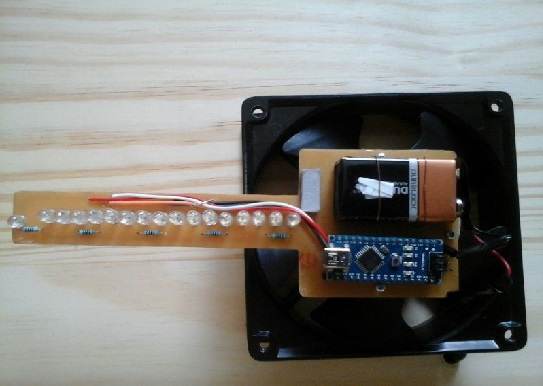
\includegraphics{./modelo_final.jpg}
	\caption[Modelo final do projeto]{Modelo final do projeto}
	\label{fig:modelo_final}
\end{figure}

Utilizando este modelo, foi possível obter um ótimo resultado estético no projeto. A placa e o motor, juntos com a bateria para alimentação dos componentes eletrônicos, encaixaram perfeitamente no hardware desenvolvido pela equipe. Porém, devido à limitações físicas, não foi possível combinar com sucesso a programação do software com o que foi construído. O algoritmo desenvolvido para o funcionamento do relógio funciona perfeitamente se as limitações do hardware forem desconsideradas, e pode ser usado em novos projetos.

Juntando as duas partes do trabalho (software e hardware) foi possível visualizar os ponteiros e a borda do relógio, entretanto, os ponteiros não ficaram fixos na posição em que deveriam estar, pois o número de rotações por minuto do motor estava variando de acordo com as condições físicas do relógio.

Realizando vários testes empíricos foi possível observar que o software funcionou de maneira correta e que a variável que não estava com o comportamento esperado era o número de rotações por minuto. A base do motor não estava completamente fixa, causando uma pequena trepidação em todo o sistema, a potência do motor era muito grande para que houvesse a estabilidade desejada. Na próxima secção deste trabalho serão apresentadas as conclusões da equipe a respeito das soluções para o problema.

%---------- Terceiro Capitulo ----------
\chapter{Conclusão}
\label{chap:concl}

Os objetivos sugeridos neste projeto não foram alcançados integralmente. Após analisar os resultados pudemos tirar várias conclusões, levantar as causas dos principais problemas e até mesmo sugerir soluções para a continuidade deste projeto ou desenvolvimento de trabalhos similares.

O cronograma proposto foi cumprido em sua maior parte, contudo, quando foi criado pela equipe, não previa os problemas mecânicos que surgiram ao longo do desenvolvimento do projeto. O resultado obtido apresentou limitações na parte física que não permitiram que o efeito final fosse visualizado de forma correta. Foi possível criar os ponteiros e as bordas do relógio, porém, tivemos dificuldades em mantê-los na posição desejada.

Com base no exame dos experimentos empíricos realizados após o projeto ter sido concluído, foi possível apurar as causas e determinar exatamente onde estava o erro. Percebemos que, devido à alta taxa de rotações por minuto do motor, não havia estabilidade suficiente no sistema, conforme a base tremia, o número de RPM mudava. Mesmo após termos fixado a base da melhor maneira que pudemos, a velocidade das hélices ainda variava demasiadamente, impossibilitando o software de funcionar como deveria. Para resolver este problema poderia ser utilizado um motor com menos potência, porém esta solução apresentaria um risco à imagem final exibida nos LED's, uma vez que existe uma frequência mínima para que o relógio seja visto perfeitamente à olho nu. Poderia também ter sido adicionado ao projeto um sensor de interrupção, indicando as rotações do motor. Desta forma o algoritmo teria que ser levemente modificado para que os LED's piscassem exatamente no momento e na posição certa, utilizando como referência, além do tempo, os dados retornados pelo sensor.

Um resultado positivo que foi apresentado nos testes é o do algoritmo desenvolvido pela equipe. Quando não existem limitações físicas, o software funciona corretamente. No futuro, se outros projetos equivalentes forem realizados, este relatório pode ser utilizado como referência neste quesito.

Para continuidade deste projeto seria necessária a implementação de um sensor de interrupção, semelhante ao tacômetro desenvolvido no início do trabalho. Desta forma, o número de rotações por minuto do motor, juntamente com a hélice, seria completamente supervisionado pelo Arduino, possibilitando uma maior precisão na posição dos LED's.

Apesar de não ter sido concluído completamente, este projeto trouxe resultados satisfatórios para toda a equipe, introduzindo novos conteúdos e apresentando desafios que testaram a capacidade dos alunos envolvidos.


%---------- Referências ----------
\bibliography{reflatex} % Geração automática das referências a partir do arquivo reflatex.bib

\apendice
%%---------- Apêndices (opcionais) ----------
\chapter{Nome do Apêndice} 

\anexo
% ---------- Anexos (opcionais) ----------
\chapter{Código completo do Relógio de Varredura Mecânica}

\begin{lstlisting}
/* chamada que acende o ponteiro dos minutos
 * deve ser chamada com os grupos 1, 2, 3 e 4 com o
 * seguinte comando:
 * blinkMin(g1_a, g2_a, g3_a, g4_a);
*/
void blinkMin (int g1, int g2, int g3, int g4)
{
      //acende os leds
      digitalWrite(g4,LOW);
      digitalWrite(g3,LOW);
      digitalWrite(g2,LOW);
      digitalWrite(g1,LOW);
      //mantem acesos pelo tempo de piscagem
      delay(pisca);
      //apaga os leds
      digitalWrite(g4,HIGH);
      digitalWrite(g3,HIGH);
      digitalWrite(g2,HIGH);
      digitalWrite(g1,HIGH);
}

/* chamada que acende o ponteiro da hora
 * deve ser chamada com os grupos 3 e 4, com o
 * seguinte comando:
 * blinkHora(g3_v, g4_v);
*/
void blinkHora (int g3, int g4)
{
      //acende os leds
      digitalWrite(g4,LOW);
      digitalWrite(g3,LOW);
      //mantem aceso pelo tempo de piscagem
      delay(pisca);
      //apaga os leds
      digitalWrite(g4,HIGH);
      digitalWrite(g3,HIGH);
}

/* funcao que incrementa o horario apos um minuto */
void incrementaHorario()
{
      //incrementa os minutos
      minuto++;

      //se for 60min, tem que zerar os min e incrementar as horas
      if(minuto == 60)
      {
            minuto = 0;
            hora++;

            //se a hora for igual a 12, zera
            if(hora == 12)
                hora = 0;
      }
}

/* funcao que faz tudo acontecer... faz com que os leds mostrem
 * um relogio usando as funcoes blinkHora e blinkMin

 * eh dividida em tres partes.. se o ponteiro das horas esta na
 * frente do dos minutos, se o dos minutos esta na frente ou se
 * estao alinhados. isso depende de saber qual o angulo entre os
 * ponteiro e a origem (o eixo vertical, apontando diretamente pra
 * cima).
 */
void clock ()
{
      //calcula o angulo do ponteiro em relacao a origem
      int ang_min = minuto*6;

      //calcula o angulo do ponteiro das horas
      int ang_hora = (hora*30) + (minuto/2);

      //se o ponteiro das horas estiver antes dos minutos
      if (ang_hora < ang_min)
      {
             //diferenca de tempo entre os ponteiros
             int atraso_entre = ((ang_min-ang_hora)*arco_min);

             /*tempo entre o ultimo ponteiro de uma volta e o primeiro da
             proxima*/
             int atraso_apos = ((360-ang_min+ang_hora)*arco_min);

             //delay entre a origem e o primeiro ponteiro
             int atraso_antes = hora*arco_min;

             //aguarda o tempo entre a origem e o primeiro ponteiro
             delayMicroseconds(atraso_antes);

             //loop que pisca os ponteiro sequencialmente 2400 vezes
             //variavel contadora
             int n = 0;

             for(n=0; n<rpm; n++)
             {
                   blinkHora(g3_v, g4_v);
                   delayMicroseconds(atraso_entre);
                   blinkMin(g1_a, g2_a, g3_a, g4_a);
                   delayMicroseconds(atraso_apos);
             }

             //apos um minuto (2400 voltas) chama a funcao novamente
             clock();
      }

      //se o ponteiro dos minutos esta antes das horas
      else if (ang_min<ang_hora)
      {
             //diferenca de tempo entre os ponteiros
             int atraso_entre = ((ang_hora-ang_min)*arco_min);
             /*tempo entre o ultimo ponteiro de uma volta e o primeiro da
             proxima*/
             int atraso_apos = ((360-ang_hora+ang_min)*arco_min);
             //delay entre a origem e o primeiro ponteiro
             int atraso_antes = minuto*arco_min;

             //aguarda o tempo entre a origem e o primeiro ponteiro
             delayMicroseconds(atraso_antes);

             //loop que pisca os ponteiro sequencialmente 2400 vezes
             //variavel contadora
             int n = 0;

             for(n=0; n<2400; n++)
             {
                   blinkMin(g1_a, g2_a, g3_a, g4_a);
                   delayMicroseconds(atraso_entre);
                   blinkHora(g3_v, g4_v);
                   delayMicroseconds(atraso_apos);
             }

             //apos 1min roda a funcao mais uma vez
             clock();
      }

      else
      {
            int atraso_antes = ang_min*arco_min;
            int atraso_apos = 360*arco_min;

            //loop
            int n = 0;
            for(n=0; n<2400; n++)
            {
                  blinkHora(g3_v, g4_v);
                  blinkMin(g1_a, g2_a, g3_a, g4_a);
                  delayMicroseconds(atraso_apos);
            }

            clock();
      }
}

/*
 * programa que torna um trilho de leds girando em um relogio usando o
 * fenomeno da POV.

 * as saidas pares sao verdes, as impares sao azuis e a borda eh
 * vermelha

 * o ponteiro das horas eh verde e o dos minutos eh azul
*/


int hora = 13;
int minuto = 50;

int rpm = 2400; //valor medido de rotacoes por minutos
int arco_min = 416; //valor do arco de 1min (6 graus) em micros

int accel = 0; /*valor para o cooler acelerar e posicionar a placa
na posicao norte (apontada para cima), em s*/

int pisca = 0; //valor que um led fica aceso ao piscar, em micros


//da nome para as saidas de cada grupo
int g4_v = 12;
int g4_a = 11;
int g3_v = 10;
int g3_a = 9;
int g2_v = 8;
int g2_a = 7;
int g1_v = 6;
int g1_a = 5;
int borda = 4;


void setup()
{
      //seta os pinos como saidas
      pinMode(g4_v,OUTPUT);
      pinMode(g4_a,OUTPUT);
      pinMode(g3_v,OUTPUT);
      pinMode(g3_a,OUTPUT);
      pinMode(g2_v,OUTPUT);
      pinMode(g2_a,OUTPUT);
      pinMode(g1_v,OUTPUT);
      pinMode(g1_a,OUTPUT);
      pinMode(borda,OUTPUT);

      //desliga os leds
      digitalWrite(g4_v,HIGH);
      digitalWrite(g4_a,HIGH);
      digitalWrite(g3_v,HIGH);
      digitalWrite(g3_a,HIGH);
      digitalWrite(g2_v,HIGH);
      digitalWrite(g2_a,HIGH);
      digitalWrite(g1_v,HIGH);
      digitalWrite(g1_a,HIGH);
      digitalWrite(borda,HIGH);
}

void loop ()
{
      //tempo entre ligar o arduino e colocar o cooler na tomada, em s
      delay(5000);

      //tempo para o cooler acelerar ate a posicao de origem
      delay(accel);
      //loading();
      clock();
}
\end{lstlisting} 

\end{document} 